\chapter{Drasil}
\label{c:drasil}

\ds{**Section Roadmap:
    -- This is where the real meat of Drasil is discussed (implementation details)
    -- Intro to our knowledge-capture mechanisms
      - Chunks/hierarchy
      - Break down each with examples from the case studies.
      - Look for 'interesting' examples (synonyms, acronyms, complexity, etc.)
    -- Intro to the DSL
      - Captured knowledge is useless without the transformations/rendering engine
      - DSL for each \sf{}}

In this chapter we introduce the Drasil framework and some details of its 
implementation including knowledge-capture mechanisms, the domain specific 
languages used throughout, and how all of these pieces are brought together in 
a human-usable way to generate \sfs{}. The name Drasil, derived from Norse 
Mythology's world tree Yggdrasil whose branches spread across the 
many realms, is representative of how our framework spreads across the many 
domains and contexts relevant to software generation.
      
\section{Drasil in a nutshell}

Manually writing and maintaining a full range of \sfs{} is redundant, tedious, 
and often leads to divergent \sfs{}. Drasil is a purpose-built framework 
created to tackle these problems.

Contrary to documentation generators like Doxygen, Javadoc, and Pandoc
which take a code-centric view of the problem and rely on manual redundancy -- 
i.e. natural-language explanations written as specially delimited
comments which can then be weaved into API documentation alongside code -- 
Drasil takes a knowledge-centric, redundancy-limiting, fully traceable, single 
source approach to generating \sfs{}.

However, Drasil is not, nor is it intended to be, a panacea for all the woes of 
software development. Even the seemingly well-defined problems of unnecessary 
redundancy and manual duplication turn out to be large, many-headed beasts 
which exist across a multitude of software domains; each with their own 
benefits, drawbacks, and challenges.

To reiterate: Drasil has not been designed as a silver-bullet. It is a 
specialized tool meant to be used in well-understood domains for software that 
will undergo frequent maintenance and/or changes. In deciding whether Drasil 
would be useful for developing software to tackle a given problem, we recommend 
identifying those projects that are long-lived (10+ years) with \sfs{} 
relevant to multiple stakeholders. For our purposes, as mentioned earlier, we 
have focused on SC software that follows the input $\rightarrow$ process 
$\rightarrow$ output pattern. SC software has the benefit of being relatively 
slow to change, so models used today may not be updated or invalidated for some 
time, if ever. Should that happen, the models will likely still be applicable 
given a set of assumptions or assuming certain acceptable margins for error.

With Drasil being built around this specific class of problems, we remain aware 
that there are likely many in-built assumptions in its current state that could 
affect its applicability to other domains. As such, we consider expanding 
Drasil's reach as an avenue for future work.

The Drasil framework relies on a knowledge-centric approach to software 
specification and development. We attempt to codify the foundational theory 
behind the problems we are attempting to solve and operationalize it through 
the use of generative technologies. By doing so, we can reuse common knowledge 
across projects and maintain a single source of truth in our knowledge database.

Given how important knowledge is to Drasil, one might think we are building 
ontologies or ontology generators. We must make it clear this is \emph{not} the 
case. We are not attempting to create a source for all knowledge and 
relationships inside a given field. We are merely using the information we have 
available to build up knowledge as needed to solve problems. Over time, this 
may take on the appearance of an ontology, but Drasil does not currently 
enforce any strict rules on how knowledge should be captured, outside of its 
type system and some best practice recommendations. We will explore knowledge 
capture in more depth in Section~\ref{sec:kc}.

\section{Our Ingredients: Organizing and Capturing Knowledge}
\label{sec:kc}

For Drasil to function as intended, we need a means of capturing and organizing 
the underlying knowledge of the software systems we are trying to build 
alongside common knowledge that would be relevant across our entire target 
domain of SC software. This knowledge capture method must also be robust enough 
to be operationalized by a multi-faceted generation framework.

Before we can design a knowledge capture mechanism, we must first define what 
exactly we believe we need to capture. It is nearly impossible to consider 
every case of knowledge that could be used in the domain of SC software, not to 
mention an extremely large undertaking to begin with ``all the things". As 
such we have decided to take an iterative, progressive refinement approach to 
our knowledge capture mechanisms. This should come as no surprise and follows 
from our general process for developing the Drasil framework.

\subsection{Capturing Knowledge via Chunks}
\label{sec:kcChunk}

We begin by borrowing and re-purposing the \emph{chunk} term from Literate 
Programming (LP) and use it to create a simplified, extensible, and ever 
expanding hierarchy  of chunks based on the requirements for capturing a single 
piece of knowledge. Our base chunk, \codeH{NamedChunk} is defined in 
Figure~\ref{fig:namedchunk} and can be thought of as any uniquely identifiable 
term. It is composed of a \codeH{UID}, or unique identifier, and a 
\codeH{NP}, or noun phrase, representing the term.

\fig{
\lstinputlisting[language=Haskell, firstline=33, lastline=43, 
firstnumber=33]{code/NamedIdea.hs}}{NamedChunk Definition}{fig:namedchunk}

A single node does not a hierarchy make, but with the root \codeH{NamedChunk} 
defined, we can begin to progressively extend it to cover any new chunk types 
we may need for our knowledge capture requirements. For example, if we want to 
capture a simple term with its definition, we need more than just a 
\codeH{NamedChunk}. We need to extend \codeH{NamedChunk} to include a 
definition, and we refer to this particular variant chunk as a 
\codeH{ConceptChunk}. For ease of creation, we define a number of semantic, 
so-called \emph{smart constructors} for each chunk type which allow us to more 
simply define our chunks and their intermediary datatypes (ie: \codeH{UID} and 
\codeH{NP} from the \codeH{NamedChunk} example). An example of such smart 
constructors being used to create simple instances of \codeH{ConceptChunk} can 
be seen in Figure~\ref{fig:conceptchunk}. Note there are smart constructors 
for each datatype when multiple variants exist and could be used in a given 
place. Looking at the \codeH{ConceptChunk} example, we can see two different 
smart constructors (\codeH{cnIES} and \codeH{cn'}) being used to create the 
\codeH{NP} instance. Both smart constructors create an instance of \codeH{NP}, 
but in this case the smart constructor used defines given properties (ie. 
pluralization rules of the noun phrase used as a term) for the instance to 
simplify construction.

\fig{
\lstinputlisting[language=Haskell, firstline=76, 
lastline=82, firstnumber=76]{code/Math.hs}}{Some example instances of 
\codeH{ConceptChunk} 
using the \codeH{dcc} smart constructor}{fig:conceptchunk}

These simple chunks are fine as a starting point, however, knowing the SC 
domain we can already foresee the need for a variety of other chunks. For 
brevity, we will only expand upon the chunks needed for the examples used in 
this paper. More information, including detailed definitions of all the types 
and current state of Drasil can be found in the wiki 
(\href{https://github.com/JacquesCarette/Drasil/wiki/}
{https://github.com/JacquesCarette/Drasil/wiki/}) or the Haddock documentation 
which can be generated from the Drasil source code or found online at 
\href{https://jacquescarette.github.io/Drasil/docs/full/}
{https://jacquescarette.github.io/Drasil/docs/full/}

\subsection{Chunk Combinatorics}
\label{sec:chunky}
\ds{Would we call our chunk hierarchy a DSL? Or would the DSL be more along the 
lines of Expr and Sentence which make up our chunks?}

Even with extremely simple chunks we have seen the need for multiple chunk 
types and a number of ways to construct instances of those types. The more we 
extend our chunk hierarchy, the larger the number of possible combinations we 
will need to account for. This is not only relevant to chunks themselves, but 
also to the information they encode. Take, for instance, a term definition that 
relies on other terminology that has been captured. In our effort to reduce 
duplication and maintain a single source of information, we intend to be able 
to create chunks with references to other chunks such that the definition can 
use the known terminology.

\ds{Should I work in something about how we use lenses in here, as all complex 
chunks are instances of the simpler chunks they've been built from? Or is that 
getting too into the Haskell-specific details?}

To define a term with references to other terms, we need to ensure we are 
creating our definitions by projecting relevant knowledge into the definition, 
but also ensuring we have the flexibility to extend that knowledge. With that 
in mind, we created a Domain Specific Language (DSL) for creating and combining 
(English language) sentences aptly called \codeH{Sentence}. In its most basic 
form, \codeH{Sentence} will simply wrap a string. However, by defining a number 
of helper functions and other useful utilities, our \codeH{Sentence} DSL can be 
used to combine, change case, pluralize, and more. A simple example of a series 
of chunks that utilize the \codeH{Sentence} DSL to derive their definitions can 
be seen in Figure~\ref{fig:acceleration}. We use the \codeH{phrase} helper 
function to pull the appropriate sentence out of the \codeH{velocity} chunk and 
the combinator (\codeH{+:+}) to concatenate the sentences. Note that position 
uses a different smart constructor (for non-derived definitions) and so doesn't 
require the sentence constructor (\codeH{S}) around its definition.

\fig{
\lstinputlisting[language=Haskell, linerange={59-60,135-136,174-175}, 
numbers=none]{code/Physics.hs}
}{Projecting knowledge into a chunk's definition}{fig:acceleration}

Looking back at our examples of the types of knowledge we are interested in 
from Figure~\ref{fig:gbrddq} we can see that the simple chunks we've defined so 
far do not even start to cover the full spectrum of our needs. We can see a lot 
of information missing such as a symbolic representation ($\hat{q}$) and 
equation ($\hat{q} = \frac{q(ab)^2}{Eh^4\text{GTF}}$). As that is a relatively
complex example, we will start by looking at something far simpler: Newton's 
2nd Law of motion\citep{Newton1687} which, roughly translated, states ``the net 
force on a body at any instant of time is equal to the body's acceleration 
multiplied by its mass or, equivalently, the rate at which the body's momentum 
is changing with time"  or as most physics students recognize it $F=ma$ 
provided we have definitions for $F$, $m$, and $a$.

To understand what exactly is missing, let us look at how we achieve an 
operational definition of \emph{Force} as a chunk in Drasil. To start, we can 
see we need a symbolic representation ($F$) and some way to define an equation. 
Also, each of force, mass, and acceleration are measured in some form of units 
($N$, $kg$, and $m/s^2$ respectively) which we will likely care to capture and 
keep track of. 

\fig{
\lstinputlisting[language=Haskell, linerange={91-92}, 
firstnumber=91]{code/Physics.hs}
}{The force \codeH{ConceptChunk}}{fig:forceCC}

\fig{
\lstinputlisting[language=Haskell, linerange={47-47,57-57}, 
numbers=none]{code/PhysicsQuantities.hs}
}{The force and acceleration \codeH{UnitalChunk}s}{fig:forceUC}

We start by building a \codeH{ConceptChunk} for the Force concept as seen in 
Figure~\ref{fig:forceCC}. It is built from a common noun (``force") and a 
definition. Next we need to capture the units of measurement to the force 
concept by defining what we have named a \codeH{UnitalChunk}. This definition 
for force can be seen in Figure~\ref{fig:forceUC}. Note that we are not 
re-defining force in this instance. We are instead using a smart constructor to 
build atop the existing force chunk (\codeH{CP.force}) and adding a symbolic 
representation (\codeH{vec cF}, which is shorthand for the selected vector 
representation\footnote{More on this in Section~\ref{sec:recipes}} of the 
capital letter \emph{F}). We also must capture the units used to measure force
(\codeH{newton}) which are defined in \codeH{Data.Drasil.SI_Units} and can be 
seen in Figure~\ref{fig:Data.Drasil.SI}. The SI Units are captured using 
another type of chunk known as a \codeH{UnitDefn} which are built atop a 
\codeH{ConceptChunk} and \codeH{UnitSymbol}. The \codeH{UnitSymbol} is also a 
chunk that can be one of several other chunk types.\footnote{For brevity we are 
glossing over many chunk definitions and the differences between them as there 
are a large variety in use for even simple examples. They are covered in more 
depth in the full technical documentation found on our github repository.}. 
Returning to the force \codeH{UnitalChunk}, the smart constructor \codeH{uc} we 
are using will assume we are working in the real number space. There are 
other smart constructors for other spaces, which are also captured using other 
chunks elsewhere in Drasil (see: \codeH{Language.Drasil.Space}).

\fig{
\lstinputlisting[language=Haskell, linerange={21-30}, 
firstnumber=21]{code/SI_Units.hs}
}{The fundamental SI Units as Captured in Drasil}{fig:Data.Drasil.SI}

\fig{
\lstinputlisting[language=Haskell, linerange={11-20}, 
firstnumber=11]{code/PhysicsUnits.hs}
}{Examples of chunks for units derived from other SI Unit chunks}{fig:accelU}

Now we approach the terms mass and acceleration in a similar manner. We capture 
each as a \codeH{ConceptChunk} (see Figure~\ref{fig:acceleration} for a 
reminder of how we captured acceleration's definition relative to velocity and 
thus relative to position). Then construct a \codeH{UnitalChunk} for each. 
Acceleration can be seen in Figure~\ref{fig:forceUC} and mass has a similar 
\codeH{UnitalChunk} that uses the \codeH{metre UnitDefn} chunk. More 
interestingly, the units for acceleration are derived from other units, and can 
be seen in Figure~\ref{fig:accelU} with some additional derived unit types 
(taken from \codeH{Data.Drasil.Units.Physics}).

Now we have almost everything we need to finish our definition of Newton's 
second law. Everything thus far has been defined in natural language using our 
\codeH{Sentence} DSL, but it is not well-suited to the one piece we are 
currently missing: a way to define expressions relating chunks in a universal 
\ds{language agnostic?} (mathematics) context \ds{/representation}.

\subsection{Relating Chunks via Expressions}
\label{sec:expr}

Continuing our Newton's Second Law example from Section~\ref{sec:chunky}, we 
need a means to capture how force is calculated. We know it is calculated 
relative to mass and acceleration, so we need a way to encode that, preferably 
in an operational manner. We also know acceleration is itself derived from 
time and velocity, which is derived from time and position.

When thinking about the types of information we would like to encode with 
expressions, we have some obvious candidates. We should be able to encode 
common arithmetic operations (addition, subtraction, multiplication, division, 
exponentiation, etc.), boolean operations (and, or, not, etc.), comparisons 
(equal, not equal, less than, greater than), trigonometric functions (sin, tan, 
cos, arctan, etc.), calculus (derivation, integration, etc.), and vector/matrix 
operations (dot product, cross product, etc.). For the sake of our example 
we'll focus on only those we need to define Newton's Second Law of motion: 
multiplication and derivatives.

\fig{
\lstinputlisting[language=Haskell, linerange={194-202}, 
firstnumber=194]{code/Expr.hs}
}{Defining real number multiplication in \codeH{Expr}}{fig:mulRe}

As an aside, we will elide details on how we arrived at the current 
implementation of the expression DSL known as \codeH{Expr}, but suffice to say 
it was driven by a practical, ``lowest common denominator" approach to 
developing the operations that could be encoded and factoring out commonalities 
much the same way we did with the rest of the case studies. With that in mind, 
we have encoded multiplication (for real numbers) as seen in 
Figure~\ref{fig:mulRe}. \codeH{AssocA} refers to an associative arithmetic 
operator which can be applied across a list of expressions (in this case, 
\codeH{mulRe}, though addition and other associative operations look very 
similar). Derivation is much simpler to encode, as it is simply a relationship 
between two existing chunks, ie. \codeH{deriv a b} represents taking the 
derivative of \codeH{a} with respect to \codeH{b}.

\fig{
\lstinputlisting[language=Haskell, linerange={16-16, 20-23}, 
numbers=none]{code/PhysicsEquations.hs}
}{Encoding Newton's second law of motion}{fig:newton}

Continuing our example, we see (Figure~\ref{fig:newton}) it is fairly trivial 
to encode the expression for Newton's Second Law using the \codeH{Expr} DSL. We 
are still not done building our Newton's Second Law chunk however, as this 
specific law should be referable by its own identifier. It is not simply 
``force", nor the relationship between mass and acceleration, but a combination 
of both with its own natural language semantics that allow us to refer to it 
specifically. The full definition for this particular chunk can then be found 
in Figure~\ref{fig:newtonChunk}. The chunk is defined relative to force and the 
expression captured in Figure~\ref{fig:newton}, alongside a new identifier and 
description. Notice we are building off of other chunks throughout each piece 
of the chunk's definition, thus giving us perfect traceability from beginning 
to end, regardless of whether we are looking at a defining expression or 
natural language description.

\fig{
\lstinputlisting[language=Haskell, linerange={34-42}, 
numbers=none]{code/PhysicsEquations.hs}
}{Newton's second law of motion as a \emph{Chunk}}{fig:newtonChunk}

The \codeH{Expr} DSL grants us flexibility in defining relationships without 
imposing any particular structure on a chunk other than ``contains an 
\codeH{Expr}", or more specifically ``can be modeled using an \codeH{Expr}." 
Our example also shows us that a few simple chunk types can be combined 
repeatedly to build much more robust, complex, and information-dense chunks. On 
the other hand, encoding even a relatively simple theory like Newton's Second 
Law of motion requires us to define chunks down to the fundamentals. 
Luckily, that is another area where chunks shine as they are infinitely 
reusable. Once a chunk has been defined and added to our knowledge-base, we 
never need to redefine it. We simply use it wherever it is needed.

On the topic of using chunks, we now need a means for taking our chunks and 
structuring them such that we can actually do something useful with them. For 
example, how would we go from chunks to \sfs{}? Look forward to that in 
Section~\ref{sec:recipes}.

\subsection{Chunk Classification}
%\ds{Prev title: ``Chunk Summary" and comment: I kind 
%of want to skip this section, though I can
%also understand keeping it. It does feel a little too ``in the weeds" to go 
%through the whole Chunk Hierarchy, but I do think it's worthwhile to include
%the kinds of things we can capture. Maybe a brief ``We've touched on Blah, and 
%we've also determined we need to be able to capture `blerb, flerb, and 
%gerb'"(Constraints or something).}

\ds{I've modified this section to not only be called something different, but 
to get into the weeds a bit on chunk classification, so we can show the high 
level ``Class of chunk has this property" instead of ``Here are all our chunk 
datatypes"}

In the previous sections, we used the idea of ``chunks" of knowledge as our 
building blocks. They range in complexity from simple single terms, to complex 
relationships between expressions and overarching conceptual frameworks. Each 
chunk is useful for a particular encoding, and complex chunks are built from 
simpler, more fundamental chunks. With all of the complexities of mixing and 
matching chunks, we have developed a need for a way to determine which chunks 
expose the same types of knowledge (and how they differ). Not only would such a 
system ease our ability to develop new chunks, by avoiding repetition and 
ensuring the new chunk is uniquely suited to its purpose, but it 
also aids in our understanding of which chunks are suited to capture what types 
of knowledge.

We have developed a classification system for chunks grouping them based on 
the properties they encode. For example, all chunks encoding things that are 
measured with units would be instances of the \codeH{Unitary} type. Chunks that 
capture quantities, whether Unitary or not, 
would be instances of the \codeH{Quantity} type. As we simplify, we end up 
determining what qualifies something as a chunk in the first place. That is, 
what is the root property that \emph{all} chunks must have to be considered a 
chunk? That is the \codeH{HasUID} classification, which essentially states that 
a given chunk of knowledge can be referred to by some unique identifier. For a 
more intuitive example, the \codeH{NamedIdea} classification is used 
for chunks that encode knowledge represented by given terms such as ``force", 
``computer", ``priority", and so on.

Figure~\ref{fig:chunkClasses} and Figure~\ref{fig:chunksClassified} show a 
subset of the different ways we classify chunks and some example chunk types 
and how they would be classified, respectively. Note there is a one to many 
relationship between a given chunk and its classifications. \ds{Use UnitalChunk 
and DefinedQuantityDict in the figure to show how they differ, yet are 
classified into many of the same types} As you can see, the \codeH{UnitalChunk} 
and \codeH{DefinedQuantityDict} are very closely related in that they both 
contain their own \codeH{NamedIdea}, \codeH{Space}, \codeH{Symbol}, and 
\codeH{Quantity}, however, the \codeH{UnitalChunk} is also classified as 
\codeH{Unitary} as it \emph{must} have a unit associated with it.

\fig{\begin{center}
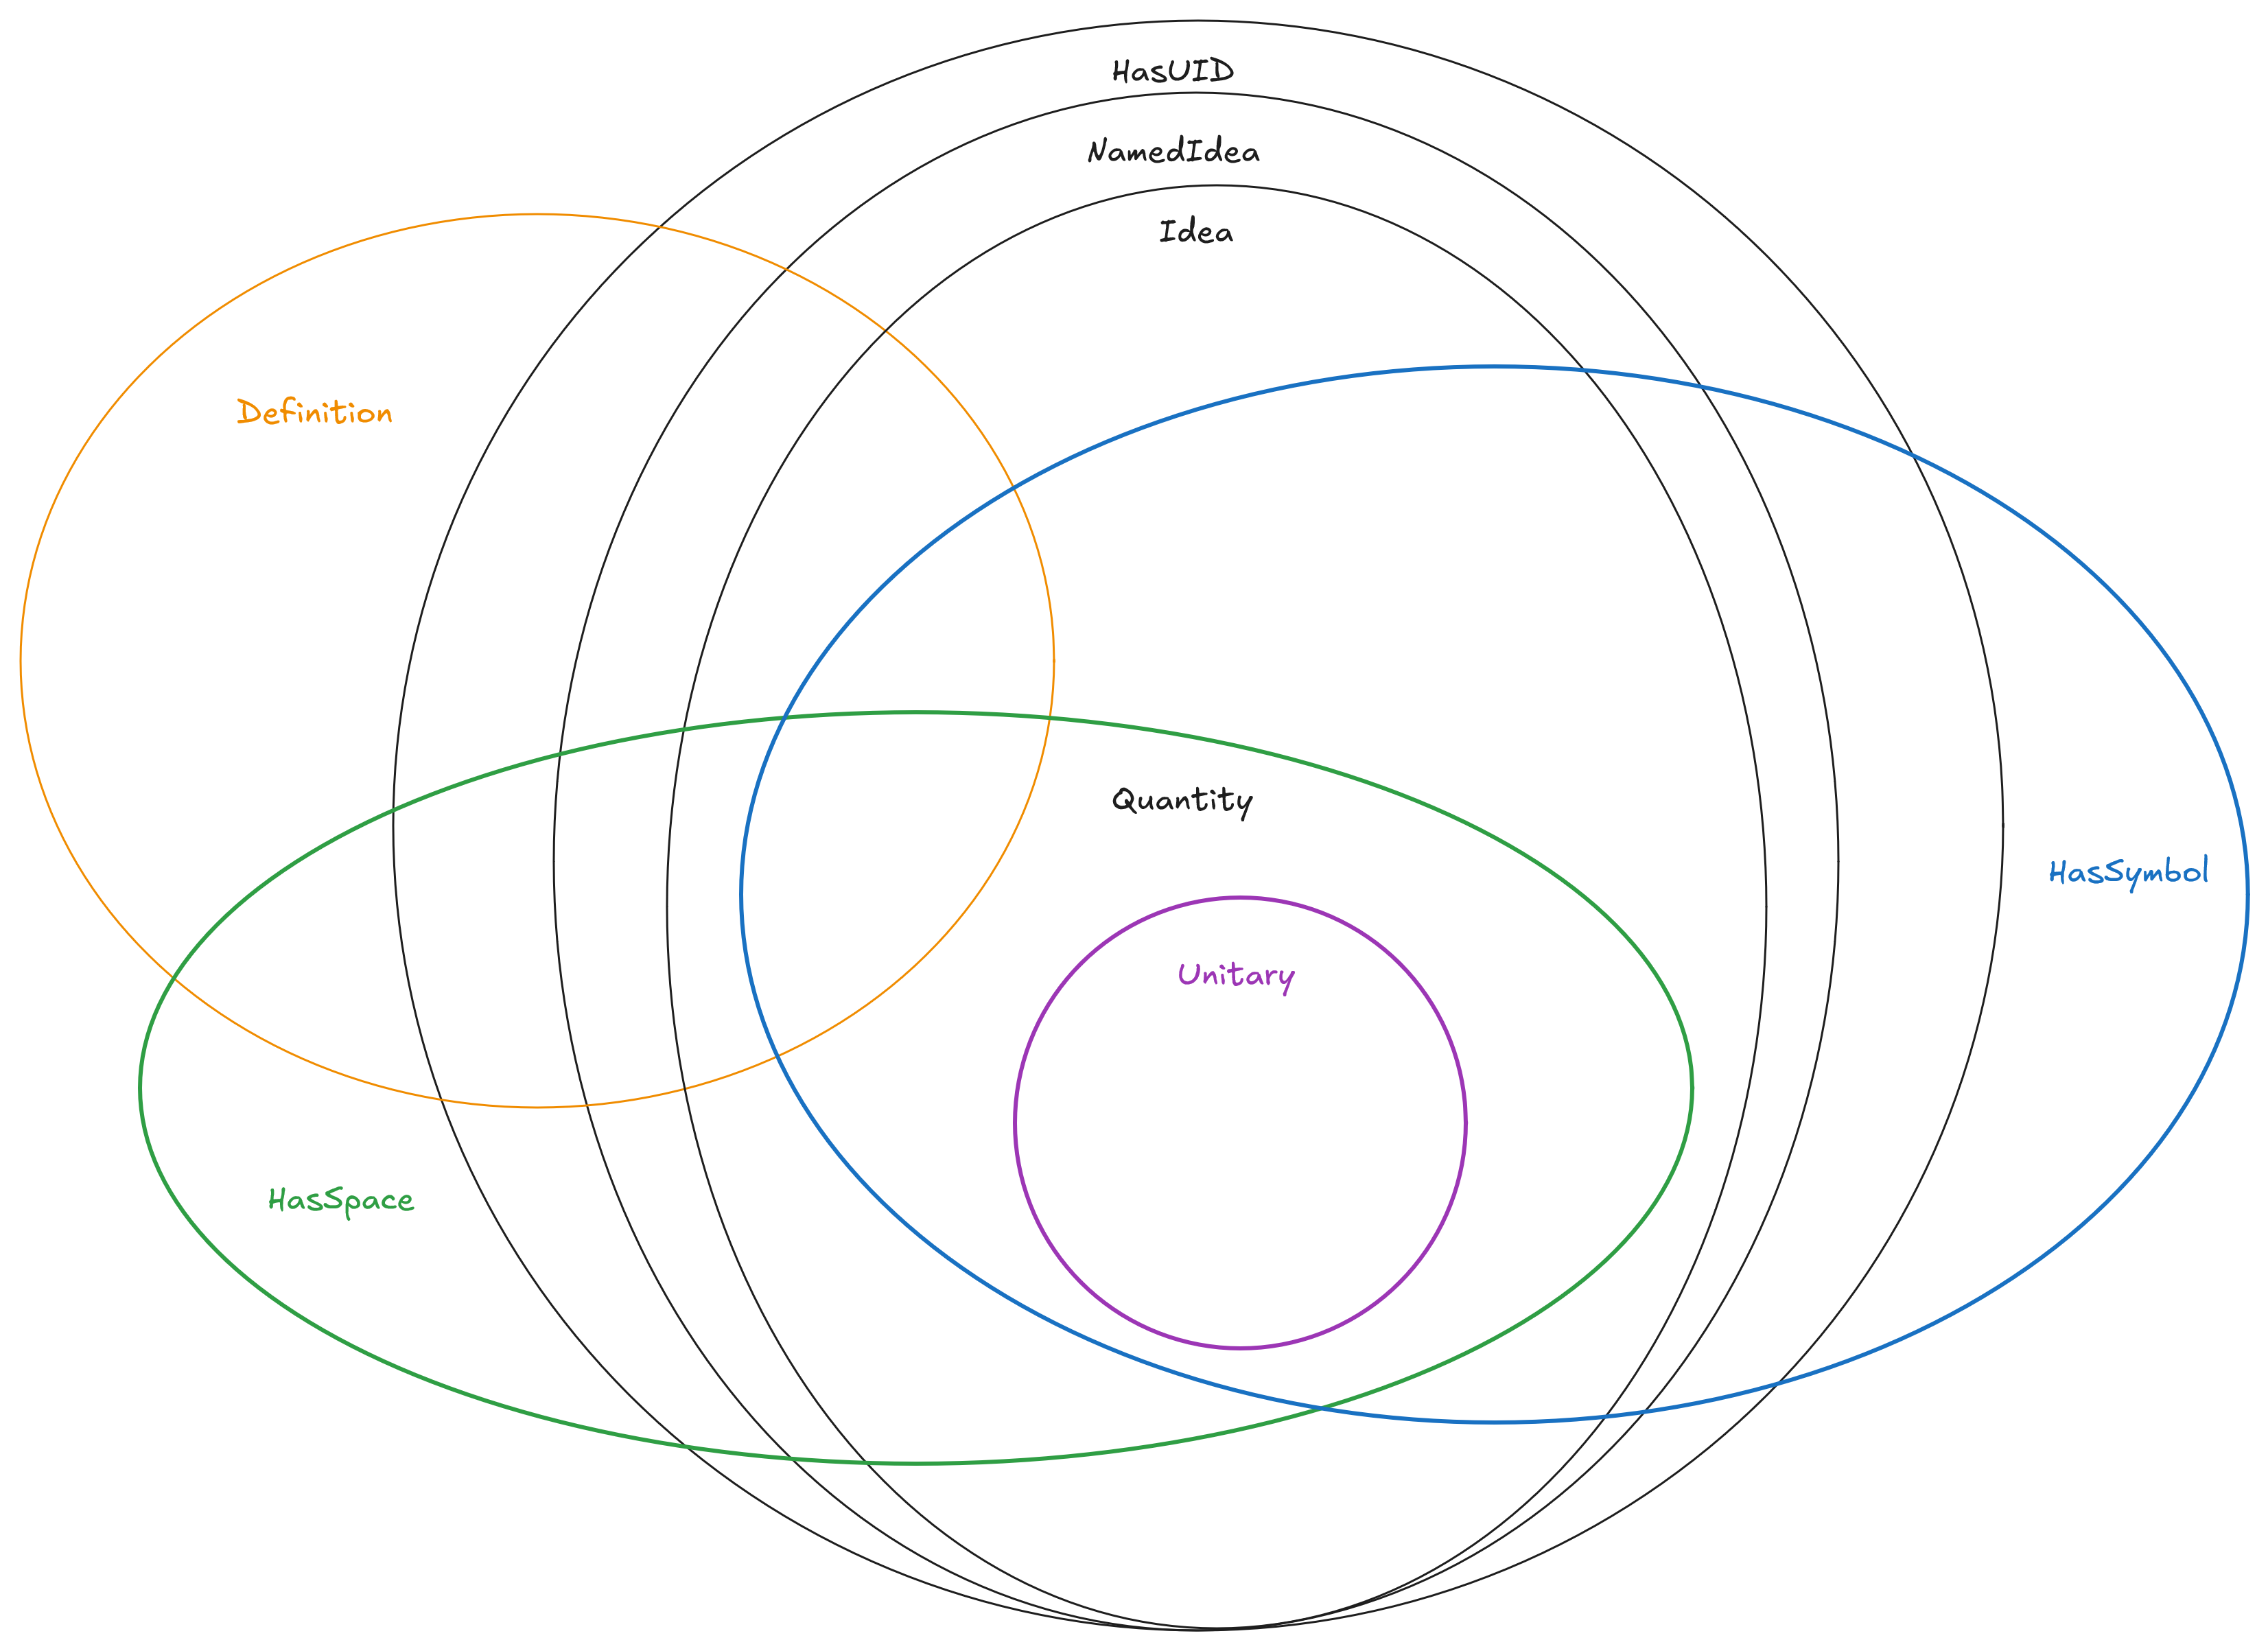
\includegraphics[width=\linewidth]{figures/ChunkClasses.png}
\end{center}}{A subset of Drasil's Chunk Classification system showing some of 
the encoded property relationships}{fig:chunkClasses}

\fig{\begin{center}
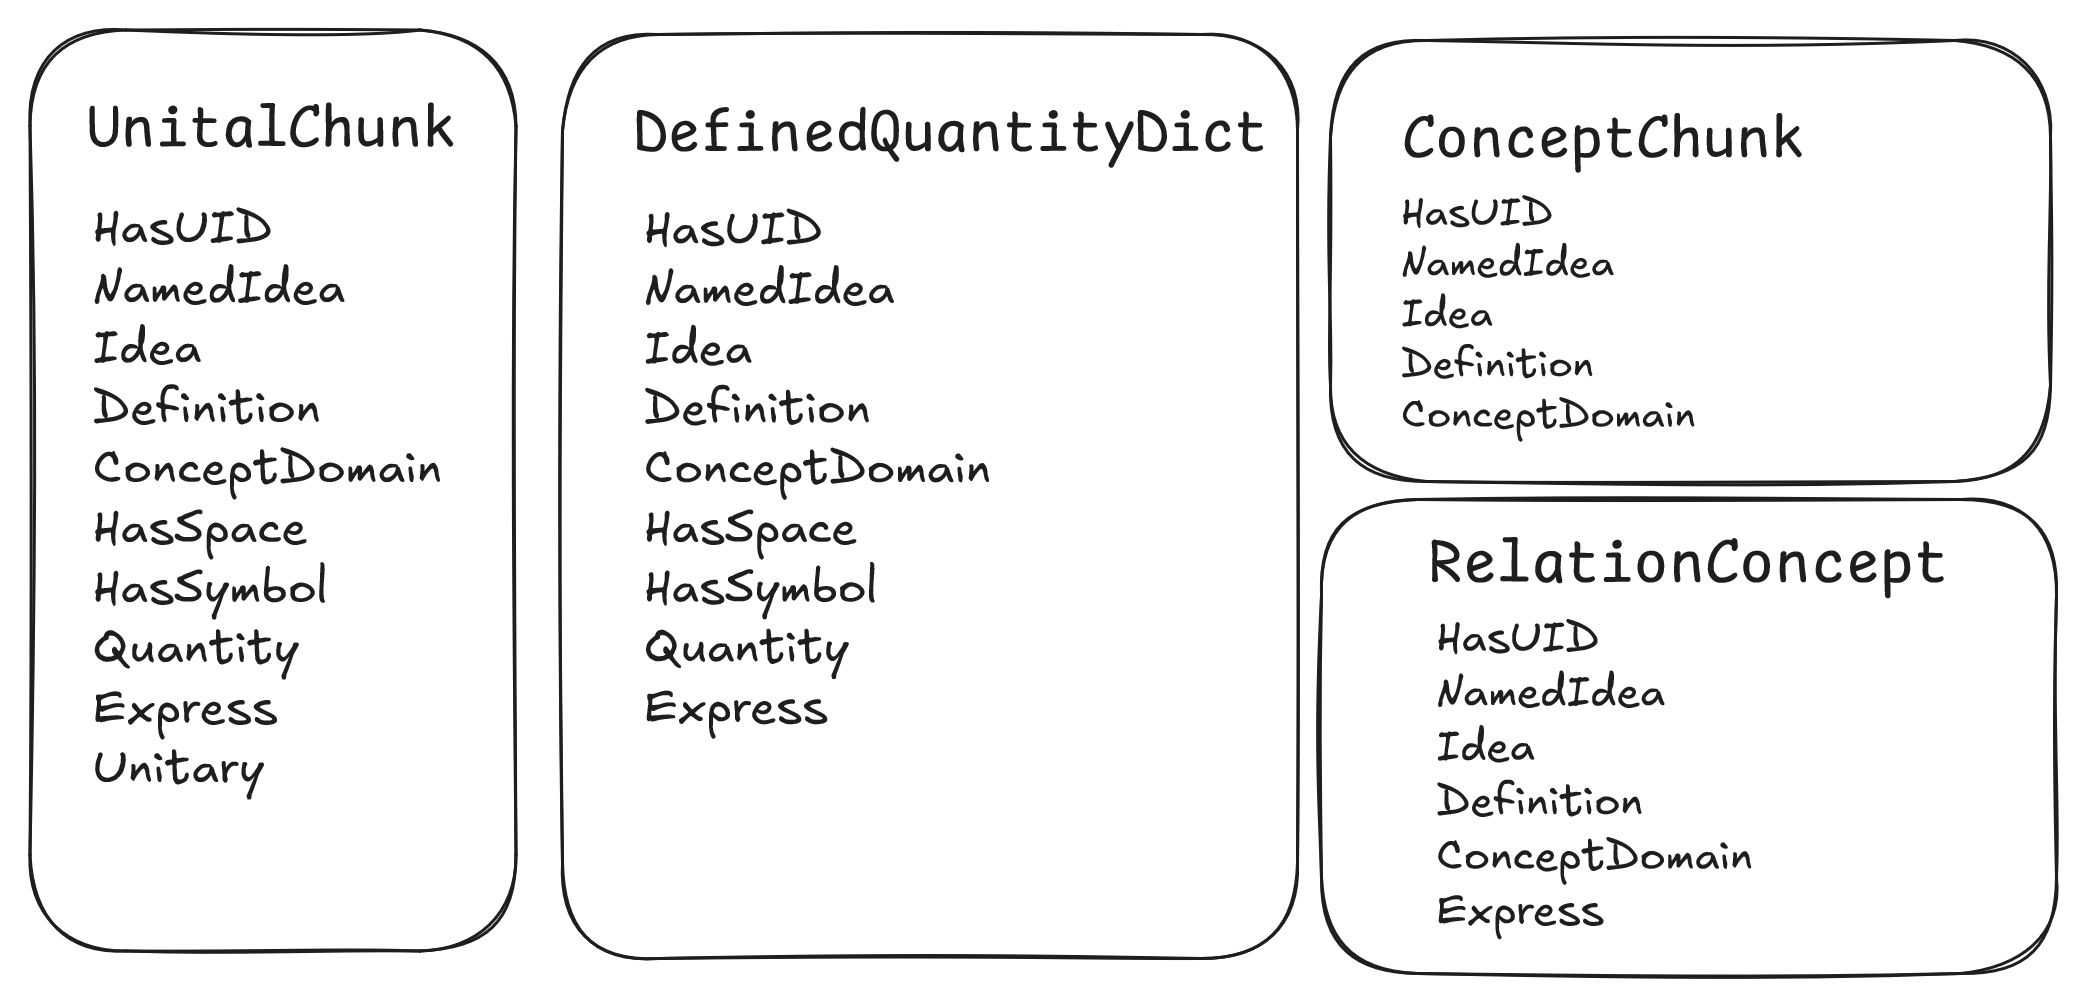
\includegraphics[width=0.75\linewidth]{figures/ChunkClassified.png}
\end{center}
}{A subset of Drasil's chunks showing how different chunks may belong to 
multiple classifications}{fig:chunksClassified}

\ds{I need something at the end here to finish up the section (for flow), but 
something like ``With the ability to create unique chunks based on the 
properties tied to the given underlying knowledge being encoding we are finally 
ready to take things a step further and figure out how to use them." seems 
redundant as I start the next section with basically the same line}


\section{Recipes: Codifying Structure}
\label{sec:recipes}

Now that we have a means of encoding and organizing knowledge, we need some 
way to operationalize it. Our knowledge base is essentially just a collection 
of chunks, which are themselves a collection of definitions, encoded in our 
Expr and Sentence DSLs. To generate \sfs{} we need a means to define the 
overall structure of the \sf{} as well as the knowledge projections we require 
to expose the appropriate knowledge from our chunks in a meaningful way for the 
target audience of that particular \sf{}. This is where our \emph{Recipe} DSL 
comes into play.

A recipe is, in it's simplest form, a specification for one or more \sfs{}. 
It is an intermediate representation of a given \sf{} and can be thought of as 
a ``little program". With it, we select which knowledge is relevant and how it 
should be organized before passing the recipe to the generator/rendering engine 
to be consumed and produce the final \sf{}. A recipe not only allows us to 
structure where knowledge should be presented, but also gives us tools for 
automatically generating non-trivial sections of our \sfs{}. For example, a 
traceability matrix can be automatically generated by traversing the tree of 
relationships between chunks within a recipe, although we'll discuss that in 
more depth in Section~\ref{sec:gen}.

As we saw in Section~\ref{sec:patterns}, there are patterns of repetition for 
the way knowledge is projected and organized within and between our \sfs{}. The 
recipe DSL has been designed to take advantage of our knowledge capture 
mechanisms to reduce unnecessary repetition and duplication. We consider the 
\sfs{} as different views of the same knowledge, and project only that which is 
relevant to the audience of the specific \sf{} our recipe applies to. For 
example, a human readable document may use symbolic mathematics notation for 
representing formulae whereas the source code would represent the same formulae 
using syntax specific to the programming language in use (or, taking an extreme 
example in the case of punch cards, punched cards). Regardless, we would define 
the underlying knowledge once in our chunks, and use the recipe DSL to select 
the representation.

\ds{A little repetitive above, but wanted to really hammer in what recipes are 
for.}

As our case studies are following templates for our \sfs{}, they give us a 
solid foundation with which to write our recipes. We already know how the 
knowledge should be organized, greatly simplifying how we can begin structuring 
our recipe DSL. The most straightforward, practical approach would be to start 
by defining a recipe for a given \sf{} type (SRS, MG, Code, etc.). Then flesh 
that out section by section, following the template as an organizational guide, 
using the patterns we discovered earlier (Section~\ref{sec:patterns}) as a 
means of avoiding unnecessary duplication. This is the approach we have chosen 
to follow, and it has lead to some interesting results.

\fig{
\codeBlock{DocDecl}{25}{42}
}{Recipe Language for SRS}{fig:recipeSRS}

As an example, let us take a look at the recipe language we have defined 
\ds{What do we call 
this? I mean the generic recipe for SRSes, not the specific example of glassbr 
or w/e} for an SRS using the \smithea{} template.
Looking at the \codeH{DocSection} definition from Figure~\ref{fig:recipeSRS}, 
we can see a striking resemblance to (a subset of) the template's 
Table of Contents (Figure~\ref{fig:SRSToC}). Each section is defined by a 
datatype, which is, through a similar mechanism, decomposed into multiple 
subsections (for example, Figure~\ref{fig:recipeReqSec} shows the decomposition 
of the requirements section) which then defines the types of organizational 
structures we use for specifying the contents of a given subsection. When 
populated, the recipe specifies both the structure of our expected \sf{} and 
the knowledge (chunks) contained therein.

\fig{
\codeBlock{DocDecl}{88}{98}
}{\codeH{ReqrmntSec} Decomposition and Definitions}{fig:recipeReqSec}

As the given recipe so far has provided nothing but structure, you may be 
wondering how we populate it with the appropriate knowledge chunks to produce a 
\sf{}? For that, we should look at a specific example from one of our case 
studies (\gb{}).

\subsection{Example: SRS recipe for \gb{}}
\label{sec:glassBRSRSRecipe}

\fig{
\codeBlock{Body}{54}{55}
\vdots{}
\codeBlock{Body}{85}{126}
}{SRS Recipe for \gb{}}{fig:glassBRSRSRecipe}

The recipe for the \gb{} SRS can be seen in Figure~\ref{fig:glassBRSRSRecipe}.
This should look familiar, as it follows a similar structure to the \smithea{} 
template table of contents. We use a number of helper functions and data types 
to condense and collect the chunks we require and avoid writing any generic 
boilerplate text. The structure of the document can be rearranged to an extent, 
in that we can add, remove, or reorder sections at will by simply moving them 
around within the \codeH{SRSDecl}. We can also make choices regarding the 
display of certain types of information in the final, generated \sf{}. For 
example, we alluded to vector representations earlier 
(Section~\ref{sec:chunky}) which we currently can display using either bold
typeface or italics. This choice must be made using the \codeH{TypogConvention} 
datatype which lists the choices made (ex. 
\codeH{TypogConvention[Vector Bold]}) and is used by a relevant portion of the 
SRS recipe if vectors are included in the \sf{}. Our \gb{} example does not 
make use of this convention, however the \gp{} case study does.

As for the chunks necessary for generating the \sf{}, each section includes 
references to them through supplied lists in something we call the 
\code{C}{System Information} %System is a Haskell kw
object (Figure~\ref{fig:systemInformation}).

\fig{
\codeBlock{Body}{63}{81}
}{System Information for \gb{}}{fig:systemInformation}

The system information object uses helper functions to keep track of the lists 
of chunks necessary for filling in the sections of our \sf{}, the SRS. Each 
piece of the object consists of one or more chunks to be used in filling in the 
relevant sections. A quick description of each property can be found in 
Table~\ref{tab:siBreakdown}, but it should be noted that some of the defined 
properties are only there for convenience (and/or remain only until the next 
refinement pass) as they are derived from other chunks with the use of 
helper functions and could be inferred.

\ds{TODO: I might remove the table and just add comments to the code block 
similar to 
what's in the next section. It seems like that might be easier for readers to 
reference}

\begin{table}[]
\caption{System information object breakdown - every property is represented by 
chunks encoding given information}
\label{tab:siBreakdown}
\begin{tabular}{| P{.2\linewidth} | p{.8\linewidth}|}
\hline
 \textbf{Property} & \textbf{Chunk(s) Referenced}


\\ \hline
	\_sys & System name (ex. "\gb{}").


\\ \hline
	\_kind & \SF{} type we are defining (ex. SRS).


\\ \hline
	\_authors & List of authors of the \sf{}.


\\ \hline
	\_purpose & Purpose of the \sf{}.


\\ \hline
	\_quants & List of required quantities.


\\ \hline
	\_concepts & List of required concepts not otherwise encoded.


\\ \hline
	\_instModels & List of required instance models.


\\ \hline
	\_datadefs & List of required data definitions.


\\ \hline
	\_configFiles & List of required configuration files.


\\ \hline
	\_inputs & List of required inputs to the system.


\\ \hline
	\_outputs & List of required outputs from the system.


\\ \hline
	\_constraints & List of constraints for the system (physical and software 
	specific).


\\ \hline
	\_constants & List of required constants. 


\\ \hline
	\_sysinfodb & Database of all required symbols. \ds{confirm this}


\\ \hline
	\_usedinfodb & Database of all used acronyms and symbols. \ds{confirm this}


\\ \hline
	refdb & Database of all relevant external references/citations.

	
\\ \hline
\end{tabular}
\end{table}
 
As should be obvious, the system information object is referencing other chunks 
which have been defined elsewhere. Most definitions can be found in the 
knowledge-base, with system-specific aggregations (i.e. lists of chunks) being 
defined within the scope of the specific example project. For example, 
\codeH{iMods} referenced as the \codeH{_instModels} property is defined 
as shown in Figure~\ref{fig:iMods}, alongside the two system-specific instance 
models listed within it. The two specific instance models can be seen to be 
derived from other existing chunks, through the use of a series of helper 
functions, thus ensuring their traceability to the knowledge-base.

\fig{
\codeBlock{IMods}{18}{19}
\vdots{}
\codeBlock{IMods}{28}{33}
\vdots{}
\codeBlock{IMods}{41}{46}
}{The \codeH{iMods} definition}{fig:iMods}

Given that the system information object refers to all of the requisite chunks 
for the knowledge contained in our \sfs{} and the SRS recipe defines how that 
knowledge should be structured and organized within the \sf{}, it follows that 
those are all we should need to generate our SRS. As an aside, the complete 
recipe for the SRS specification of \gb{}\footnote{Not including chunks 
referenced from within our knowledge bases as they can be shared, reused, and 
are not necessarily specific to only this system.} including the system 
information object is contained in a single file in less than 370 lines of 
code\footnote{Including many comments, whitespace, and import statements.}. 
Teasing our results: the generated SRS in PDF format is 44 pages in length. 
This is partially due to our ability to strip away all of the common 
boilerplate text that we need not worry about right now, as that will be a 
problem for the generator (Section~\ref{sec:gen}). As it stands we have created 
the recipe language to represent what we truly want out of a recipe: a 
simplified, unnecessary-duplication-avoiding, fully traceable representation of 
our target \sf{}.

With the combination of system information and the SRS recipe we can soon move
on to creating our generator for the finished SRS document. As the other \sf{} 
recipes were developed in tandem with the SRS, they follow a similar structure 
and in the interest of brevity we will skip the breakdown of each recipe. It is 
left to the reader to investigate them by diving into our examples via the 
Drasil github. However, there is one \sf{} that is significantly different, and 
as such, we will go into more depth in discussing in the following section: the 
executable code recipe. Said recipe allows us to not only specify knowledge and 
the way we wish it structured, but also implementation choices that we would 
like to make in the final generated source code.

\ds{TODO ? (SEE BELOW COMMENT) - basically the list is obviously referencing 
other things, which are themselves defined elsewhere, and we can follow that 
through to figure out wtf is going on. I will pick one (DD) and traverse the SI 
to show how things (ex. GTF) are defined. It'll be a bunch more code snippets.}
\ds{Changed my mind on the above, I think the current example is shorter and 
flows more easily. The chunk definitions aren't relevant to the recipe lang 
itself or its definition, all that's relevant is that they exist. The generator 
/ final generation example should follow a single DD throughout as described in 
the above comment.}

\subsection{Example: Executable Code recipe for \gb{}}

\ds{I've gone back and forth a few times on this and can't think of a good way 
to give the executable code recipe for \gb{}. I might need to rethink the way 
I do it / go for the previous section's approach}

\ds{the below is the generic CodeSpec DSL, not the \gb{} one. TODO: fix that, 
and use the CodeSpec stuff the same way we used System information above.}

As mentioned in the previous section, the executable code is a significantly 
different \sf{} than the documentation-heavy \sfs{} we've already discussed. We 
have created a recipe language for executable code, and an example (taken from 
GlassBR) can be seen in Figure~\ref{fig:gbCodeRecipe}.

The recipe DSL for the executable code (\codeH{CodeSpec}) is fairly 
straightforward, even though the executable code is so different from the other 
\sfs{} in both style and audience. The DSL itself can be seen in 
Figure~\ref{fig:codeSpec}. If you squint, it looks fairly similar to the system 
information object, albeit with a few distinct differences. There are many 
references to modules, which we have not yet explicitly discussed. We will look 
into them in a bit more depth in Section~\ref{sec:gen}, but for now suffice to 
say they have their own DSL for tying the various requisite chunks together.

\fig{
Body.hs
\codeBlock{Body}{57}{58}
Choices.hs
\codeBlock{Choices}{13}{27}}{The Recipe for \gb's Executable 
Code}{fig:gbCodeRecipe}

\fig{
\codeBlock{CodeSpec}{41}{72}
}{The Recipe Language for Executable Code (CodeSpec)}{fig:codeSpec}



\section{Cooking it all up: Generation/Rendering}
\label{sec:gen}
  - Recipes are “little programs”
  - Each recipe can be rendered a number of ways, based on parameters fed to the generator.
  -  Implicit parameters vs explicit: Ex. an SRS will always be rendered based on the recipe, but its output will either be LaTeX or HTML based on an explicit choice. Implicit params fed to gen table of symbols/A\&A / ToU.


\section{Iteration and refinement}
\label{sec:iterefine}
\ds{TODO: Figure out what belongs here and what belongs in results}

  - Practical approach to iron out kinks / find holes in Drasil

  - Find places to improve upon the existing case studies - ‘update as you go’ 
  mindset

  - Observe the amount of effort required to correct errors - show examples

  - Tau example (see issue 348) and its implications - symbols and definitions 
  didn't match. -> implicit 1m depth into the page (means we may need to change 
  the equations). Resistive and mobilizing shear switched throughout the 
  original docs -- impossible with Drasil.

  - \ds{This next one might belong in future work} Implicit assumptions -> 
  Issue 91. We take for granted things are "physical 
  materials", but this is an assumption that could be codified and made 
  explicit to the system (which would allow us some more flexibility).